\documentclass[12pt, conference]{IEEEtran}

\usepackage{cite}
\usepackage{amsmath,amssymb,amsfonts}
\usepackage{algorithmic}
\usepackage{graphicx}
\usepackage{textcomp}
\usepackage{xcolor}
\usepackage{float}
\def\BibTeX{{\rm B\kern-.05em{\sc i\kern-.025em b}\kern-.08em
    T\kern-.1667em\lower.7ex\hbox{E}\kern-.125emX}}

\begin{document}

\title{Sudoku Slayer}

\author{\IEEEauthorblockN{Alice Hanigan}
\and
\IEEEauthorblockN{John Summers}
}

\maketitle

\begin{abstract}

The use of Constraint Satisfaction Problems(CSP) for modeling and solving Sudoku Puzzles is a natural implementation of CSP techniques.
Genetic Algorithms(GA) offer a much broader approach to the search space, but are not traditionally employed to solve Sudoku puzzles due to the puzzles structure naturally lending itself to other algorithms.
The size of a Sudoku's search space is considerable and because of this, we decided to compare the use of CSP and GA's for solving Sudoku puzzles.

\end{abstract}

\section{introduction}

Sudoku Puzzles provide a novel problem to test AI solvers against due to the simple rules and expansive search tree.
It has already been shown that Sudoku can already be categorized as NP-complete [2], and as such can be used to exhaustively test methods used in artificial intelligence.
In our project, we aimed to compare the efficacy of two approaches: using Constraint Satisfaction Problem(CSP) methods and Genetic Algorithm(GA) methods.
CSP methods have already been used to model and solve Sudoku [1] and provide a baseline for our examination of GA methods.
GA's provide a more flexible framework for describing Sudoku, relying on multiple independent variables to tailor the characteristics of the evolution between generations.
By manipulating those variables, we explore how well GA's perform we applied to a problem atypical for their application.

\section{Literature Review}

\subsection{Solving Sudoku as a CSP}

Simonis explains the history of using puzzles to examine constraint problem methodologies, citing famous puzzles such as the N-Queen and Five-Houses puzzles as well as the Minesweeper game [1].
Modeling these puzzles examines the efficacy of constraint problems methods and highlights edge-case weaknesses.
For example, while the implementation of backtracking search may solve a puzzle, it can result in an excess of comparisons resulting from overlapping constraints that arise in puzzles whose individual members have a large number of neighbors.
Sudoku is a perfect example of one such puzzle, as each cell in a traditional Sudoku has ${3n}$ neighbors, where ${n}$ is the grid-size of the ${n*n}$ puzzle.
Simonis goes onto to propose the "shaving" technique which prunes the domain of each neighbor cell as values are tested [1].
This results in a continuous reduction of the search space as arc-consistency is enforced during backtracking search and will eliminate redundant consistency checks as values examined during recursion will always be consistent will previous assignments.

\par
This pruning is desirable due to the difficulty of examining any given Sudoku with the Another Solution Problem(ASP)[2].
Yato and Seta describe the problem of determining if the solution to any given puzzle is unique, or if there exist multiple solutions.
They prove that Sudoku or "Number Place" puzzles are ASP-complete, meaning there exists some solution that is polynomial-time computable in relation to the size of its input [2].
Furthermore, ASP-completeness is shown to necessarily imply NP-completeness, meaning that computing all other elements of the search space is prohibitive.
This proof demonstrates the importance of a "shaving" technique as described by Simonis in order to efficiently solve Sudoku puzzles.

\subsection{Solving Sudoku with GA}

It is crucial, in designing a GA, to choose parameters which best fit the problem to be solved.
Ahmad Hassanat [3] writes that there are four such parameters used by GA: crossover rate, mutation rate, population size, and the number of generations.
Due to computational constraints, we were limited in our options for population size and number of generations, and as such we turned our focus primarily towards adjusting the mutation and crossover rates.

\par
We also needed to consider what methods to use in designing our GA; specifically, we needed to decide on a method for each of evaluation, selection, crossover, and mutation.
In order to better determine which methods to use, we turned towards previous experiments with and evaluations of GA.
Nisha Saini [4] states that the most commonly-used selection methods are Roulette Wheel Selection, Rank Selection, Tournament Selection, and Boltzmann Selection.
Of these, only Roulette and Tournament Selection were offered through the Python library we used, and so we considered the advantages and disadvantages of these methods.
Roulette Wheel Selection suffers from premature convergence [4], and additionally, as we discovered ourselves, is poorly-suited to minimization problems, as it favors individuals with high fitness values.
This left Tournament Selection, which preserves population diversity at the cost of degrading convergence speed [4].

\par
Mutation is a necessary complement to crossover, as it allows the GA to escape from local optima that it otherwise would be constrained to [3].
Finding the ideal mutation rate, we were surprised to find, required considering more factors than we had expected: population size, crossover rate, and number of generations all are variables in determining the best mutation rate [3].
In fact, Hassanat proposes a dynamic approach, one which increases the mutation rate and decreases the crossover rate with each generation.
Considering the complexity that Hassanat describes in this evaluation of mutation rates, we chose to focus on a set population size and crossover rate, in order to better tune our algorithm, and to create a stable environment in which to compare the respective approaches we used.

\par
Another variable that we discovered, one which we had never considered could be changed, was the number of parents used in crossover.
Traditionally, crossover is performed between two "parent" data operands, but Eiben [5] proposes a method by which crossover is performed between three or more parents.
This method, although not a new theory, has seen little practical analysis as of yet [5], and as such, we believe this would be a fascinating subject to explore if we were to extend this project.
However, to keep within our limited scope for this project, we chose to focus on binary operators for crossover.

\section{Methodology}

While CSP's are traditionally used to model Sudoku puzzles, the efficacy of GA's when solving problems with larger state spaces is undeniable.
We assume that modeling a Sudoku puzzle as a CSP will perform better when $n$ is smaller.
Our goal is to test whether or not GA's will outperform a CSP implementation when $n$ becomes larger.

\subsection{Constraint Problem Methodology}
We implemented a custom representation for traditional ${n*n}$ Sudoku puzzles in python, using dictionaries to map individual cells to their respective value, domain, and neighbors.
Simonis's "shaving"[1] technique was enforced during the initialization of our Sudoku objects.
By using shaving with a recursive search, this meant that every value we tested from a cell's domain to imply arc-consistency with its preceding layers.
Cells were chosen using "Minimum Remaining Value" criteria.
This allowed for the maximum number of values to be pruned from neighboring domains early in the search process, and minimized the number of potential assignments that any one branch could test as well as the overall depth of our search tree.
Values were only assigned to the original Sudoku object when a subsequent recursive function call passed its goal-check, at which point the return statement would bubble-up the function calls, assigning the cell : value pair it was currently testing.

\par
Our data set was obtained from an online source [6] and consisted of puzzle : solution pairs for ${9*9}$ Sudoku.
We converted this data from strings of integers to lists of integers for compatibility with our Sudoku Class.
The solutions to the puzzles were converted the same way, and correctness was checked by comparing the having our Sudoku class export a list of it's current values and then comparing that list with the list representing the known solution.
By using the same standard for both input and output data representations, not only was it simple to edit values of known cell's indices, but initialize Sudoku objects with the new value.

\subsection{Genetic Algorithm Methodology}
We used the Deap python library as the framework for organizing our GA [6].
Deap allows for the use of custom data types and functions for interfacing with the GA framework.
These custom functions effectively created our own API for the Sudoku class we had created for the CSP implementation.
This API allowed us to test various parameters for our genetic algorithm and attempt to optimize our functions for solving Sudoku puzzles.

\par
For our initial population of 10 $n*n$ Sudoku objects who's values were randomly generated.
In order to evaluate the fitness of any given Sudoku, we checked the number of constraints that its current configuration broke.
For each broken constraint, we assigned a score of -1.
The cumulative score was then the fitness value of the Sudoku, and the goal of the GA was to maximize the negative value (e.i. scores closer to 0 were more desirable).
We selected parents using the tournament selection method using the 4 fittest members of the generation.
We crossed both parents using the included cxTwoPoint function provided by the Deap library.
This performed a two point crossover of both parent's and returned two children for the next generation.
The resultant generation would be comprised of the children and members of the current generation selected via the same tournament selection method used to chose parents.
This process was repeated for the number of iterations specified by a initial parameter.

\par
We experimented with varying several parameters: the number of generations the GA was run for, the rate that "noise" was incorporated during mutation, and the number of cells effected during "noisy" mutation event.
By changing the number of generations calculated, we could weigh the effect cross-over vs. mutation on the fitness value of our final generation.
The mutation parameters were chosen because they gave us the greatest control over the ability of the GA to encounter values that may not be present in the initial population.

\par
For data, used the same $9*9$ data set that we used to test our CSP solver.
We also tested how quickly our GA solver could generate a valid complete Sudoku puzzle from a random initial population.
These random examples were generated using the default random python library, assigning a random number($<n^2$) of random values($0<value<(n+1)$).

\section{Results}
We were able to solve traditional $9*9$ Sudoku puzzles with the CSP solver.
Our GA solver was able to generate a valid $4*4$ Sudoku puzzle from an initial, randomly generated population but was unable to do so for a $9*9$ solution.

All figures were generated using the matplotlib python library. Each data point represents the average weighted score of 5 runs at the corresponding x value.
The x axis always represents the independent variable we are testing, and the y-axis will always be the highest weighted-value of the final generation.

\begin{figure}[htb]
\centerline{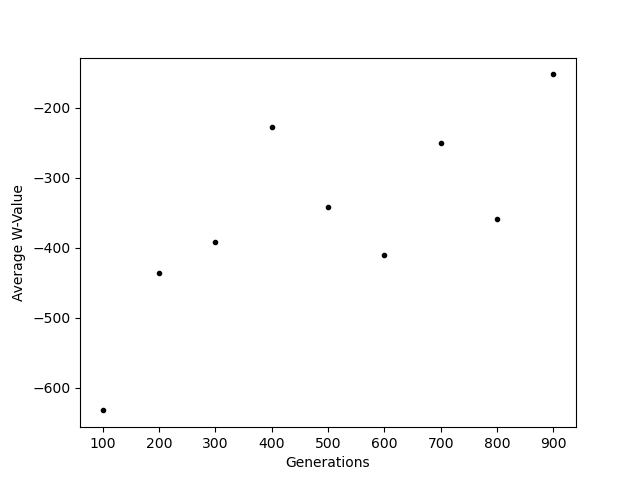
\includegraphics[scale=0.5]{Figures/Generation_Averages.png}}
\caption{The effect on increased generations on the weighted score of the final generation}
\label{fig. 1}
\end{figure}

\par
By increasing the number of generations a GA has to run, the resulting fitness of the final generation is positively effected.
It is clear that attempts to normalize values via averaging failed to produce consistent results, but a general trend can be observed.

\begin{figure}[H]
\centerline{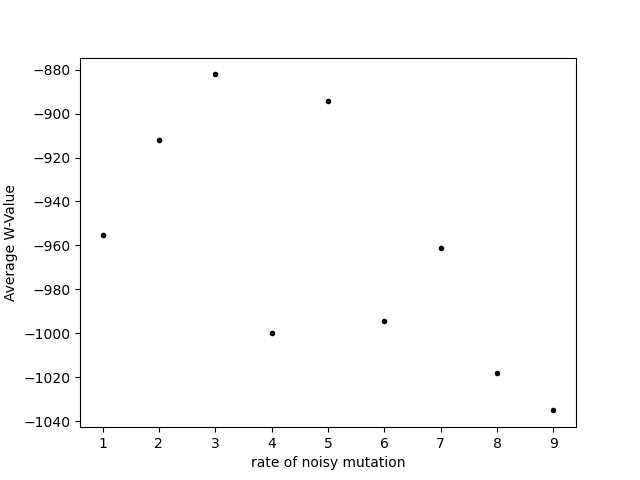
\includegraphics[scale=0.5]{Figures/Mutation_Chance_Averages.png}}
\caption{The increased rate of the addition of noise in the mutation function on the weighted score of the final generation. X axis values are the percent chance of noise being introduced.}
\label{fig. 2}
\end{figure}

\par
No correlation was found between the rate at which random values were added to a generation's children.
This could be because the increments between iterations was too large.
Another possibility could be that the chance of a "noisy" mutation needed to be less than one percent.


\begin{figure}[H]
\centerline{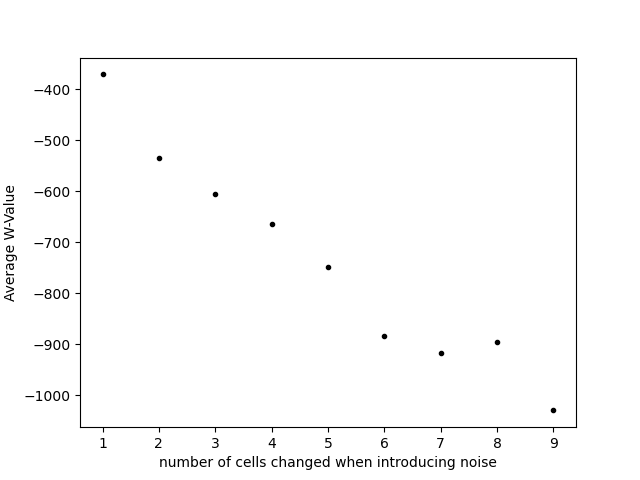
\includegraphics[scale=0.5]{Figures/Mutation_Number_Averages.png}}
\caption{The increased number of   of the addition of noise in the mutation function on the weighted score of the final generation}
\label{fig. 2}
\end{figure}

\par
The results for the number of cells changed when introducing noise suggest a negative correlation between the amount of noise introduced and the ability for the GA to control the fitness of subsequent generations.

\section{Discussion}
It is clear from our results that modeling Sudoku puzzles as a CSP provides the most robust solution for solving a Sudoku puzzle.
While GAs allow for a broader approach to problem solving, its strengths lie in its ability to derive alternate variable weightings.

\par
Our choice to vary the parameters of our GA provides insight into possible iterations on our parameters.
We believe that our results could be improved by lowering both the rate and the number of cells used when introducing noise during mutation.

\par
These results reinforce our hypothesis that CSPs are the best method for modeling Sudoku Puzzles when presented with lower $n$ values.
Higher $n$ values will cause any CSP implementation to increase in complexity, and it is still possible that GAs are able to better handle Sudoku puzzles with larger $n$ values.
Unfortunately we were unable to produce a GA that performed reliably enough to test this.

\section{Conclusion}

Although we found ourselves constrained by our circumstances in our choice of method and data, we have succeeded in creating both a deterministic algorithm that solves Sudoku puzzles as a CSP, and a genetic algorithm that solves these puzzles through evolution.
 From our research and work, we would conclude that the former is a more effective approach to such a problem, but there is still much more that could be done to explore this comparison. 
In particular, incorporating multi-parent crossover methods, implementing dynamic mutation rates, testing our methods upon other Sudoku variants (such as Killer or X Sudoku), and incorporating other emerging methods for GA would allow us to explore whether there might be more to be said on this comparison.

\begin{thebibliography}{00}

\bibitem{b1}Simonis, Helmut, 2006, "Sudoku as a Constraint Problem", http://citeseerx.ist.psu.edu/viewdoc/download?doi=10.1.1.88.2964\&rep=rep1\&type=pdf
\bibitem{b2}Tayo, Takayuki, “Complexity and Completeness of Finding Another Solution and Its Application to Puzzles”, Takahiro Seta, http://www-imai.is.s.u-tokyo.ac.jp/~yato/data2/SIGAL87-2.pdf
\bibitem{b3}Hassanat, Ahmad, “Choosing Mutations and Crossover Ratios for Genetic Algorithms-A Review with a New Dynamic Approach”,  Khalid Almohammadi, Esra’a Alkaween, Eman Abunawas, Awni Hammouri, V.B. Sura Prasath, https://www.mdpi.com/2078-2489/10/12/390/pdf 
\bibitem{b4}Nisha Saini, "review of Selection Methods in Genetic Algorithms", https://www.ijecs.in/index.php/ijecs/article/download/2562/2368/
\bibitem{b5}A. E. Eiben, “Multi-Parent Recombination”, https://www.cs.vu.nl/~gusz/papers/Handbook-Multiparent-Eiben.pdf
\bibitem{b6}

\end{thebibliography}

\end{document}
